%!TEX encoding = UTF-8 Unicode
%!TEX TS-program = xelatex
\documentclass[11pt]{article}
%% Versionning info
%%\usepackage[draft]{gitinfo2}
%% Polices OTF
\usepackage{fontspec,xltxtra,xunicode}
\usepackage{libertine}
%\setmainfont{Lucida Grande}
%% Gestion des langues
\usepackage{csquotes}
\usepackage{polyglossia}
\setdefaultlanguage{french}
\setotherlanguage{english}
%% URLs and hyperlinks
\usepackage{xcolor}
\usepackage[hyphens]{url}
\usepackage[unicode,bookmarks,colorlinks,breaklinks]{hyperref}
\hypersetup{linkcolor=blue,citecolor=blue,filecolor=blue,urlcolor=blue}
\urlstyle{same}
\usepackage[shortlabels]{enumitem}
\setlist[enumerate,1]{label=\arabic*., ref=\arabic*}
\setlist[itemize,1]{label=--,topsep=0pt,itemsep=0pt,leftmargin=*}
%% Framed boxes
\usepackage[framemethod=tikz]{mdframed}
\global\mdfdefinestyle{verif}{%
%linecolor=blue,middlelinewidth=2pt,
roundcorner=5pt,
frametitlebackgroundcolor=yellow!50!white
}
\newmdenv[style=verif,frametitle=Vérification]{verification}
%% Format de page
\usepackage{geometry}
\geometry{a4paper}
\geometry{top=25mm, bottom=30mm}
\geometry{outer=22.5mm, inner=25mm}
\geometry{foot=15mm, head=15pt}
%% Paragraphes sans indentation, légèrement espacés
\setlength{\parindent}{0pt}
\setlength{\parskip}{6pt plus1pt minus1pt}
%%
\setcounter{tocdepth}{1}
\setcounter{secnumdepth}{1}
\gappto\captionsfrench{\renewcommand{\contentsname}{Sommaire}}
%%
\makeatletter
\newcommand{\nospace}[1]{\nofrench@punctuation#1\french@punctuation}
\makeatother
%%
\usepackage{listings}
\lstset{%
  basicstyle=\footnotesize\ttfamily\nospace,breaklines=true,
  showstringspaces=false,
  commentstyle=\color{gray},
  keywordstyle=\color[HTML]{000000},
  backgroundcolor=\color[HTML]{eeeeee},
  tabsize=4,
  xleftmargin=1em,
  framextopmargin=3pt,
  framexleftmargin=1em,
  %framexrightmargin=1em,
  framexbottommargin=2pt,
  frame=bt,
  rulecolor=\color[HTML]{eeeeee},
}
%% Change footnote format to english one (back to original article.cls definition)
\makeatletter
\renewcommand\@makefntext[1]{%
    \parindent 1em%
    \noindent
    \hb@xt@1.8em{\hss\@makefnmark}#1}
\makeatother
%%
%% Illustrations
\usepackage{graphicx}
\graphicspath{{img/}}

\begin{document}

\title{Moodle sur Raspberry Pi 3\\ ou la construction d'une MoodleBox\footnote{Le présent document est mis à disposition selon les termes de la \href{http://creativecommons.org/licenses/by-nc-sa/4.0/}{Licence Creative Commons Attribution - Pas d'Utilisation Commerciale - Partage dans les Mêmes Conditions 4.0 International}.}}
%\date{11 juillet 2016\footnote{Version \gitAbbrevHash, \gitAuthorDate}}
\date{11 août 2016\footnote{Version 1.2}}
\author{Nicolas Martignoni}
\maketitle

\begingroup
\setlength{\parskip}{0pt}
\tableofcontents
\endgroup

\section{Pourquoi une MoodleBox ?}

\begin{quote}
\noindent « \emph{Et l'idée d'un petit boîtier à poser sur la table qui va déployer Moodle à toute la classe a quelque chose de magique (...)}»\footnote{Daniel Méthot, \url{https://moodle.org/mod/forum/discuss.php?d=330291\#p1332370}.}
\end{quote}

L'idée d'une MoodleBox est issue d'une discussion survenue au printemps 2016 dans les forums de la communauté francophone de Moodle\footnote{\url{https://moodle.org/course/view.php?id=20}.} autour de la mise à disposition d'une plateforme Moodle depuis un ordinateur local\footnote{\url{https://moodle.org/mod/forum/discuss.php?d=318719}.}, afin de fournir un environnement d'apprentissage même dans des régions éloignées de toute infrastructure réseau. L'idée a rapidement bourgeonné de construire une telle configuration avec un Raspberry Pi 3, et de la rendre accessible directement par Wi-Fi\footnote{\url{https://moodle.org/mod/forum/discuss.php?d=330291}.}.

Grâce à la persévérance d'un membre de la communauté\footnote{Christian Westphal, Académie de Strasbourg, voir \url{https://moodle.org/user/view.php?id=1378197&course=20}.}, une méthode de construction d'une MoodleBox a été proposée\footnote{\url{https://moodle.org/mod/forum/discuss.php?d=331170}.}. Reprenant certaines idées de cette première version, ce document décrit comment construire une MoodleBox à base d'une Raspberry Pi 3.

\section{Fonctionnalités de la MoodleBox}

\subsection{Ce que fait la MoodleBox}

\begin{itemize}
\item Point d'accès sans fil. Le nom du réseau Wi-Fi fourni est \emph{MoodleBox} ; le mot de passe de connexion est \emph{moodlebox}.
\item Interface graphique pour redémarrer et éteindre la MoodleBox, ainsi que pour régler la date et l'heure de la MoodleBox (au moyen d'un plugin d'administration de Moodle\footnote{\url{https://github.com/martignoni/moodlebox-plugin}.}).
\item Plateforme Moodle 3.1.x accessible via Wi-Fi (\url{http://moodlebox.local/}), dans sa configuration de base vierge de toute personnalisation. L'unique compte utilisateur du Moodle est un compte administrateur, nom d'utilisateur : \emph{admin}, mot de passe : \emph{Moodlebox4\$}. La plateforme est configurée pour accepter les clients de l'app mobile officielle\footnote{\url{https://download.moodle.org/mobile/}.} de Moodle. La taille maximale des dépôts de fichiers est fixée à 50~Mo. Le cron est lancé toutes les 3 minutes.
\item Lorsqu'une clef USB est insérée dans la MoodleBox, les fichiers qu'elle contient sont accessibles pour les administrateurs et enseignants de la plateforme via le dépôt \emph{Système de fichiers} du Moodle.
\item Possibilité de déposer des fichiers par SFTP directement sur la MoodleBox (nom d'utilisateur : \emph{moodlebox}, mot de passe : \emph{Moodlebox4\$}); ces fichiers sont accessibles pour les administrateurs et enseignants de la plateforme via le dépôt \emph{Système de fichiers} du Moodle.
\item Accès à Internet : si la MoodleBox est connectée par câble à un réseau relié à Internet, elle agit comme routeur et les clients Wi-Fi ont accès à Internet.
\item PhpMyAdmin installé (\url{http://moodlebox.local/phpmyadmin}), avec un compte administrateur, nom d'utilisateur : \emph{root}, mot de passe : \emph{Moodlebox4\$}.
\end{itemize}

\subsection{Ce que la MoodleBox ne fait pas}

\begin{itemize}
\item Serveur de courriel : la MoodleBox est prévue pour être utilisée «en campagne», indépendamment d'une infrastructure réseau ; la fonctionnalité de serveur de courriel n'a donc pas d'intérêt pour cet usage.
\item Machine à café : cette fonctionnalité, ainsi que l'implémentation du protocole HTCPCP\footnote{\url{https://tools.ietf.org/html/rfc2324}.}, sera mise en œuvre ultérieurement. Il n'est en revanche pas prévu d'implémenter le protocole HTCPCP-TEA\footnote{\url{https://tools.ietf.org/html/rfc7168}.}.
\end{itemize}


\section{Installation initiale de la Raspberry}

\subsection{Préparation de la carte microSD}

Télécharger l'image \emph{Raspbian Jessie Lite} depuis le site de Raspberry Pi\footnote{\url{https://www.raspberrypi.org/downloads/raspbian/}.}, puis la copier sur une carte microSD. Les procédures détaillées, qui varient suivant le système d'exploitation, sont disponibles sur le site de Raspberry Pi\footnote{\url{https://www.raspberrypi.org/documentation/installation/installing-images/}.}.

\subsection{Démarrage de la Raspberry et connexion}

Éjecter la carte microSD et l'insérer dans la Raspberry Pi, puis brancher l'alimentation de la Raspberry.

\begin{verification}
La diode rouge — indiquant la présence d'une alimentation — s'allume ; la verte, qui signale les accès à la carte microSD, clignote irrégulièrement après 1 à 2 secondes.
\end{verification}


Dès maintenant, toutes les manipulations se font en ligne de commande, par \lstinline{ssh} (\lstinline{Putty} sur Windows, terminal sur OS X ou Linux).

Connecter la Raspberry au moyen d'un câble Ethernet sur un réseau avec un serveur DHCP. La Raspberry sera dès lors accessible sur le réseau au moyen de l'adresse \lstinline{raspberrypi.local}\footnote{Cette adresse sera changée ultérieurement en \lstinline{moodlebox.local}.}.
\iffalse
Le serveur DHCP (la box par exemple) indique l'adresse IP de la Raspberry. Dans la suite du document, on suppose que l'adresse IP de la Raspberry est \lstinline{192.168.1.212}.
\fi

\begin{verification}
Depuis votre ordinateur, taper la commande \lstinline{ping -c3 raspberrypi.local}. La réponse doit être quelque chose comme ci-dessous.

\begin{lstlisting}[language=bash]
$ ping -c3 raspberrypi.local
PING raspberrypi.local (192.168.1.212): 56 data bytes
64 bytes from 192.168.1.212: icmp_seq=0 ttl=64 time=0.452 ms
64 bytes from 192.168.1.212: icmp_seq=1 ttl=64 time=0.251 ms
64 bytes from 192.168.1.212: icmp_seq=2 ttl=64 time=0.222 ms

--- raspberrypi.local ping statistics ---
3 packets transmitted, 3 packets received, 0.0% packet loss
round-trip min/avg/max/stddev = 0.222/0.308/0.452/0.102 ms
\end{lstlisting}
\end{verification}

Se connecter à la Raspberry. Le compte utilisateur est \emph{pi} et le mot de passe est \emph{raspberry} (le mot de passe sera changé plus tard, tout comme le compte utilisateur).

\begin{lstlisting}[language=bash]
$ ssh pi@raspberrypi.local
$ pi@raspberrypi.local's password:
\end{lstlisting}

\begin{verification}
Si tout ce passe correctement, vous êtes connecté à la MoodleBox et la console affiche

\begin{lstlisting}[language=bash]
The programs included with the Debian GNU/Linux system are free software;
the exact distribution terms for each program are described in the
individual files in /usr/share/doc/*/copyright.

Debian GNU/Linux comes with ABSOLUTELY NO WARRANTY, to the extent
permitted by applicable law.
pi@raspberrypi:~ $
\end{lstlisting}
\end{verification}

\subsection{Configuration initiale de la Raspberry}

Mettre à jour le système d'exploitation de la Raspberry, puis lancer l'utilitaire \emph{raspi-config}.

\begin{lstlisting}[language=bash]
$ sudo apt-get update -y
$ sudo apt-get dist-upgrade -y
$ sudo raspi-config
\end{lstlisting}

Avec l'utilitaire \emph{raspi-config}, effectuer les tâches suivantes\footnote{Cette partie est inspirée de \url{https://moodle.org/mod/forum/discuss.php?d=331170}.}:
\begin{itemize}
\item agrandir la partition à la taille maximale de la carte microSD;
\item modifier le mot de passe de l'utilisateur \lstinline{pi} (mot de passe fort\footnote{\url{https://xkcd.com/936/}.}). Pour cette image destinée à être distribuée, on choisira le mot de passe à \emph{Moodlebox4\$}.
\item régler les \emph{locales} à \lstinline{fr_FR.UTF-8};
\item régler le fuseau horaire et le pays pour le Wi-Fi;
\item changer le hostname de la Raspberry en \emph{moodlebox} ;
\end{itemize}

Dès maintenant, pour se connecter à la Raspberry, par SSH ou par SFTP, on utilisera l'adresse \lstinline{moodlebox.local}, le nom d'utilisateur \emph{pi} et le mot de passe \emph{Moodlebox4\$}.

\iffalse
\subsection{Mise à jour le microcode de Raspbian}

Par précaution, on effectue la mise à jour du microcode de Raspbian, puis redémarre la MoodleBox.

% sudo SKIP_BACKUP=1 PRUNE_MODULES=1 rpi-update
\begin{lstlisting}[language=bash]
$ sudo apt-get install rpi-update
$ sudo rpi-update
$ sudo reboot
\end{lstlisting}
\fi

\subsection[Changement de nom de l'utilisateur par défaut]{Changement de nom de l'utilisateur par défaut\footnote{Cette section est inspirée de \url{http://unixetc.co.uk/2016/01/07/how-to-rename-the-default-raspberry-pi-user/}.}}

L'utilisation de l'utilisateur par défaut \emph{pi} de la Raspberry Pi 3 ne pose aucun problème. Toutefois, par sécurité, il n'est pas conseillé d'employer un utilisateur dont le nom est universellement connu. On change donc le compte utilisateur par défaut. Le nom choisi ici est \emph{moodlebox}.

On commence par créer un compte utilisateur temporaire, \emph{tempuser}, et l'on définit son mot de passe.
\begin{lstlisting}[language=bash]
$ sudo useradd -m tempuser
$ sudo passwd tempuser
\end{lstlisting}

Ce compte utilisateur sera supprimé ultérieurement. La qualité du mot de passe n'est donc pas importante. Par facilité, on peut prendre le même que ci-dessus, \emph{Moodlebox4\$}.

L'utilisateur \emph{tempuser} est ajouté au groupe des \emph{sudoers}, pour lui permettre d'effectuer les opérations adéquates. On quitte ensuite la session.

\begin{lstlisting}[language=bash]
$ sudo usermod -a -G sudo tempuser
$ exit
\end{lstlisting}

On se connecte à la MoodleBox avec le compte \emph{tempuser} et le mot de passe \emph{Moodlebox4\$}.

\begin{lstlisting}[language=bash]
$ ssh tempuser@moodlebox.local
$ tempuser@moodlebox.local's password:
\end{lstlisting}

Une fois connecté à la MoodleBox, on commence par sauvegarder les fichiers que l'on va modifier, pour le cas où un problème surviendrait.

\begin{lstlisting}[language=bash]
$ cd /etc
$ sudo tar -czf /home/pi/authfiles.tgz passwd group shadow gshadow sudoers systemd/system/autologin@.service
\end{lstlisting}

On modifie ensuite dans les fichiers adéquats le nom de l'utilisateur, en le définissant à \emph{moodlebox}, puis change le nom du dossier.
\begin{lstlisting}[language=bash]
$ sudo sed -i.$(date +'%y%m%d_%H%M%S') 's/\bpi\b/moodlebox/g' passwd group shadow gshadow sudoers systemd/system/autologin@.service
$ sudo mv /home/pi /home/moodlebox
$ exit
\end{lstlisting}

On se connecte à la MoodleBox avec le nouveau nom et le mot de passe \emph{Moodlebox4\$}, qui n'a pas été changé.

\begin{lstlisting}[language=bash]
$ ssh moodlebox@moodlebox.local
$ moodlebox@moodlebox.local's password:
\end{lstlisting}

\begin{verification}
Si tout ce passe correctement, vous êtes connecté à la MoodleBox et la console affiche
\begin{lstlisting}[language=bash]
The programs included with the Debian GNU/Linux system are free software;
the exact distribution terms for each program are described in the
individual files in /usr/share/doc/*/copyright.

Debian GNU/Linux comes with ABSOLUTELY NO WARRANTY, to the extent
permitted by applicable law.
moodlebox@moodlebox:~ $
\end{lstlisting}
\end{verification}

Pour terminer, on supprime le compte utilisateur temporaire \emph{tempuser} et le fichier de sauvegarde:
\begin{lstlisting}[language=bash]
$ sudo userdel tempuser
$ sudo rm -rf /home/tempuser/
$ sudo rm authfiles.tgz
\end{lstlisting}

Désormais, on se connectera à la MoodleBox avec le nom d'utilisateur \emph{moodlebox} et le mot de passe \emph{Moodlebox4\$}.

\subsection{Correction d'un bogue dans Debian Jessie}

On profite de corriger un bogue qui a pour conséquence de remplir certains fichiers d'historique de la MoodleBox\footnote{Voir \url{https://anonscm.debian.org/cgit/collab-maint/rsyslog.git/commit/?id=67bc8e5326b0d3564c7e2153dede25f9690e6839}.}.

% sudo nano /etc/rsyslog.conf
\begin{lstlisting}[language=bash]
$ sudo sed -i '/# The named pipe \/dev\/xconsole/,$d' /etc/rsyslog.conf
$ sudo service rsyslog restart
\end{lstlisting}

\section[Configuration du point d'accès Wi-Fi]{Configuration du point d'accès Wi-Fi\footnote{Les configurations décrites dans cette section et la suivante sont inspirées de \url{https://frillip.com/using-your-raspberry-pi-3-as-a-wifi-access-point-with-hostapd/}.}}

\subsection{Paquetages nécessaires}

On commence par installer les paquetages requis.
\begin{lstlisting}[language=bash]
$ sudo apt-get install hostapd dnsmasq
\end{lstlisting}

\subsection{Configuration des interfaces réseau}

Il s'agit d'éviter que le client DHCP de la Raspberry récupère une adresse dynamique sur son interface Wi-Fi, risquant d'entrer en conflit avec son adresse fixe. On commence pour cela par modifier le fichier \lstinline{dhcpcd.conf}.
%\begin{lstlisting}[language=bash]
%$ sudo nano /etc/dhcpcd.conf
%\end{lstlisting}

On ajoute tout à la fin du fichier\footnote{Cette ligne doit être insérée cependant avant toute ligne \emph{interface} qui aurait été ajoutée au fichier.} la ligne
\begin{lstlisting}[language=bash]
denyinterfaces wlan0
\end{lstlisting}

On modifie ensuite le fichier \lstinline{/etc/network/interfaces} afin de configurer l'interface Wi-Fi de manière statique, en fixant son adresse IP. Pour la MoodleBox, on choisit l'adresse \lstinline{10.0.0.1}.
%\begin{lstlisting}[language=bash]
%$ sudo nano /etc/network/interfaces
%\end{lstlisting}

La partie \lstinline{wlan0} de ce fichier doit ressembler à quelque chose comme cela
\begin{lstlisting}[language=bash]
allow-hotplug wlan0
iface wlan0 inet static
    address 10.0.0.1
    netmask 255.255.255.0
    network 10.0.0.0
    broadcast 10.0.0.255
#    wpa-conf /etc/wpa_supplicant/wpa_supplicant.conf
\end{lstlisting}
Le reste du fichier n'est pas modifié.

\iffalse
Le contenu du fichier \lstinline{/etc/network/interfaces} devient alors

\lstinputlisting[language=bash]{files/interfaces}
\fi

\subsection[Configuration du point d'accès (\lstinline{hostapd})]{Configuration du point d'accès (\lstinline{hostapd})}

Modifier le contenu du fichier \lstinline{hostapd.conf}. C'est ici que l'on définit le nom du réseau Wi-Fi (SSID) et le mot de passe pour y accéder et d'autres options, comme le canal de diffusion. Le nom du réseau choisi est \emph{MoodleBox} et le mot de passe \emph{moodlebox}.
%\begin{lstlisting}[language=bash]
%$ sudo nano /etc/hostapd/hostapd.conf
%\end{lstlisting}

Contenu du fichier \lstinline{/etc/hostapd/hostapd.conf} :

\lstinputlisting[language=bash]{files/hostapd.conf}

\begin{verification}
Démarrer \lstinline{hostapd}:
\begin{lstlisting}[language=bash]
$ sudo /usr/sbin/hostapd /etc/hostapd/hostapd.conf
\end{lstlisting}

L'affichage annonce une erreur (puisque la configuration n'est pas finie), mais il doit se terminer par \lstinline{wlan0: AP-ENABLED}. Un client Wi-Fi doit pouvoir détecter le réseau Wi-Fi \emph{MoodleBox}.
\end{verification}

Il reste maintenant à définir où \lstinline{hostapd} doit chercher sa configuration au démarrage. Pour ce faire, on modifie le fichier \lstinline{/etc/default/hostapd}.
%\begin{lstlisting}[language=bash]
%$ sudo nano /etc/default/hostapd
%\end{lstlisting}

On y remplace la ligne \lstinline{#DAEMON_CONF=""} par \lstinline{DAEMON_CONF="/etc/hostapd/hostapd.conf"}.
\iffalse
Contenu du fichier \lstinline{/etc/default/hostapd} :

\lstinputlisting[language=bash]{files/hostapd}
\fi

\subsection{Configuration du serveur DHCP}

On modifie le contenu du fichier \lstinline{dnsmasq.conf}. Son contenu sera:
%\begin{lstlisting}[language=bash]
%$ sudo nano /etc/dnsmasq.conf
%\end{lstlisting}

\lstinputlisting[language=bash]{files/dnsmasq.conf}

\subsection{Configuration du routage}

On modifie le fichier fichier \lstinline{/etc/sysctl.conf}
%\begin{lstlisting}[language=bash]
%$ sudo nano /etc/sysctl.conf
%\end{lstlisting}
en dé-commentant (ou en ajoutant) la ligne
\begin{lstlisting}[language=bash]
net.ipv4.ip_forward=1
\end{lstlisting}

\iffalse
\lstinputlisting[language=bash]{files/sysctl.conf}
\fi

On saisit les lignes suivantes dans l'interface.

\begin{lstlisting}[language=bash]
$ sudo iptables -t nat -A POSTROUTING -o eth0 -j MASQUERADE
$ sudo iptables -A FORWARD -i eth0 -o wlan0 -m state --state RELATED,ESTABLISHED -j ACCEPT
$ sudo iptables -A FORWARD -i wlan0 -o eth0 -j ACCEPT
$ sudo sh -c "iptables-save > /etc/iptables.ipv4.nat"
$ sudo sh -c "echo 1 > /proc/sys/net/ipv4/ip_forward"
\end{lstlisting}

On crée ensuite le fichier {/lib/dhcpcd/dhcpcd-hooks/70-ipv4-nat}.
%\begin{lstlisting}[language=bash]
%$ sudo nano /lib/dhcpcd/dhcpcd-hooks/70-ipv4-nat
%\end{lstlisting}
Son contenu doit être le suivant.

\lstinputlisting[language=bash]{files/70-ipv4-nat}

Pour terminer, on redémarre la Raspberry.

\begin{lstlisting}[language=bash]
$ sudo reboot
\end{lstlisting}

\subsection{Test du point d'accès sans fil}

\begin{verification}
Au terme du démarrage, un client doit pouvoir surfer sur Internet après s'être connecté au réseau Wi-Fi \emph{MoodleBox} au moyen du mot de passe \emph{moodlebox}.
\end{verification}

\subsection{Publication des services mDNS}

Afin de rendre visible sur le réseau les services fournis par la MoodleBox, on crée le fichier \lstinline{/etc/avahi/services/moodlebox.service}, avec le contenu ci-dessous.
\lstinputlisting[language=bash]{files/moodlebox.service.xml}

\section{Installation du serveur web}

On va installer le serveur web nginx avec PHP et MySQL.

\subsection{Installation et configuration de nginx et PHP}

Installer les paquetages nécessaires.

\begin{lstlisting}[language=bash]
$ sudo apt-get install nginx php5-fpm php5-cli php5-xmlrpc php5-curl php5-gd php5-intl
\end{lstlisting}

\begin{verification}
Depuis un ordinateur connecté sur la MoodleBox via Wi-Fi, charger dans un navigateur l'URL \url{http://moodlebox.local/}. Une page web «Welcome to nginx on Debian!» doit s'afficher.
\end{verification}

Configurer le serveur web en modifiant le fichier \lstinline{/etc/nginx/sites-available/default}.
%\begin{lstlisting}[language=bash]
%$ sudo nano /etc/nginx/sites-available/default
%\end{lstlisting}
Son contenu sera le suivant.

\lstinputlisting[language=bash]{files/default}

La dernière ligne \lstinline{fastcgi_param} et la ligne \lstinline{client_max_body_size} permettent d'augmenter la taille maximale autorisée pour les dépôts de fichiers. Elle a été fixée, sur cette installation, à 50~Mo.

Relancer le serveur web
\begin{lstlisting}[language=bash]
$ sudo service nginx restart
\end{lstlisting}

\begin{verification}
Taper la commande
\begin{lstlisting}[language=bash]
$ echo '<?php phpinfo(); ?>' | sudo tee -a /var/www/html/info.php
\end{lstlisting}
puis lancer dans un navigateur l'URL \url{http://moodlebox.local/info.php}. La longue page des réglages PHP doit s'afficher, avec les variables \lstinline{upload_max_filesize} et \lstinline{post_max_size} sont fixées à 50~Mo.
\end{verification}

\subsubsection[Installation et configuration de MySql]{Installation et configuration de MySql\footnote{Cette section est inspirée de \url{http://www.syndrega.ch/?p=108}.}}

\begin{lstlisting}[language=bash]
$ sudo apt-get install mysql-server php5-mysql
\end{lstlisting}

Au cours de l'installation, on définit le mot de passe de l'utilisateur principal de la base de données \emph{root}. Comme plus haut,  on définira un mot de passe fort. Pour cette installation, le mot de passe est défini à \emph{Moodlebox4\$}.

\begin{verification}
Recharger l'URL \url{http://moodlebox.local/info.php}. Une section \emph{MySQL} supplémentaire doit apparaître dans la page.
\end{verification}

Créer une nouvelle base de données pour Moodle.

\begin{lstlisting}[language=bash]
$ mysql -u root -p
    > create database moodle;
    > grant all on moodle.* to 'root'@'localhost' identified by 'Moodlebox4$';
    > exit
\end{lstlisting}

\section{Installation de Moodle (enfin!)}

On installe Moodle à l'aide de Git, pour faciliter les mises à jour ultérieures. On commence donc par installer Git.

\begin{lstlisting}[language=bash]
$ sudo apt-get install git
\end{lstlisting}

\subsection{Téléchargement de Moodle}

\begin{lstlisting}[language=bash]
$ cd /var/www/
$ sudo git clone git://git.moodle.org/moodle.git
$ cd moodle
$ sudo git checkout MOODLE_31_STABLE
\end{lstlisting}
La dernière commande ci-dessus détermine la branche installée par Git. Dans ce cas, il s'agit de la version 3.1.x stable actuelle.

\subsection{Installation de Moodle}

On règle maintenant les permissions et crée le dossier de données de Moodle.
\begin{lstlisting}[language=bash]
$ cd ..
$ sudo rm -r html
$ sudo mv moodle html
$ sudo chown -R www-data:www-data html
$ sudo mkdir /var/www/moodledata
$ sudo chown -R www-data:www-data /var/www/moodledata
\end{lstlisting}

Pour terminer l'installation de Moodle, on lance dans un navigateur l'URL \url{http://moodlebox.local/} et l'on suit les indications données à l'écran. Cette phase dure plus de 10 minutes. Patience donc !

Pour cette installation, le compte administrateur a été défini avec le nom d'utilisateur \emph{admin} et le mot de passe \emph{Moodlebox4\$}.

\subsection[Configuration du cron de Moodle]{Configuration du cron de Moodle\footnote{Cette section est inspirée de \url{http://moopi.uk/}.}}

On lance le cron de Moodle toutes les 3 minutes. Pour ce faire, lancer la commande

\begin{lstlisting}[language=bash]
$ sudo crontab -e
\end{lstlisting}

et ajouter à la table des crons la ligne
\begin{lstlisting}[language=bash]
*/3 * * * * nice -n 10 ionice -c2 /usr/bin/php /var/www/html/admin/cli/cron.php
\end{lstlisting}

\begin{verification}
Dans Moodle, visiter l'administration sous \emph{Administration du site > Serveur > Tâches programmées}, vérifier que les tâches programmées se lancent régulièrement.
\end{verification}

\subsection{Correction du format des tables MySQL}

Pour corriger le format des tables éventuellement encore en format Antelope, on lance la commande

\begin{lstlisting}[language=bash]
$ sudo php /var/www/html/admin/cli/mysql_compressed_rows.php -f
\end{lstlisting}

\begin{verification}
La page \url{http://moodlebox.local/admin/environment.php} n'affiche plus l'avertissement sur la conversion des tables en format Barracuda.
\end{verification}

\section{Accès depuis Moodle aux fichiers d'une clef USB ou déposés par SFTP}

\subsection{Fichiers sur une clef USB}

On configure le montage automatique de clefs USB (quel que soit leur format), ainsi que l'accès à tous les fichiers de clefs USB branchées via le dépôt \emph{Système de fichiers} de Moodle\footnote{Si plusieurs clefs USB sont branchées à la MoodleBox, seuls les fichiers de la première clef branchée sont accessibles via le dépôt de fichiers.}.

Pour ce faire, on installe le paquet \lstinline{usbmount}, puis on crée un dossier dans le dossier de données de Moodle, et l'on crée enfin un lien depuis le point de montage de la clef USB vers ce dossier.

\begin{lstlisting}[language=bash]
$ sudo apt-get install usbmount
$ sudo mkdir -p /var/www/moodledata/repository
$ sudo chown -R www-data:www-data /var/www/moodledata/
$ sudo ln -s /media/usb /var/www/moodledata/repository
\end{lstlisting}

Il faut ensuite configurer Moodle de façon adéquate\footnote{Voir \url{https://docs.moodle.org/en/File_system_repository}.}: connecté comme administrateur sur la plateforme, on visite \emph{Administration du site > Plugins > Dépôts > Gérer les dépôts}.

Dans la ligne \emph{Système de fichiers}, on sélectionne dans le menu déroulant \emph{Activé et visible}.

\begin{figure}[!ht]
\begin{minipage}[b]{\linewidth}
\centering
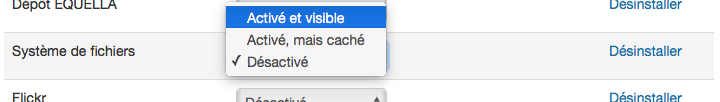
\includegraphics[width=10cm]{repo-filesystem-usb-1.png}
\end{minipage}
\end{figure}

On clique ensuite sur \emph{Enregistrer}, puis sur \emph{Paramètres} (même ligne), puis sur le bouton \emph{Créer une instance de dépôt}. Enfin, on sélectionne \emph{usb} dans le menu déroulant, et on indique \emph{Clef USB} dans le champ obligatoire \emph{Nom}.

\begin{figure}[!ht]
\begin{minipage}[b]{\linewidth}
\centering
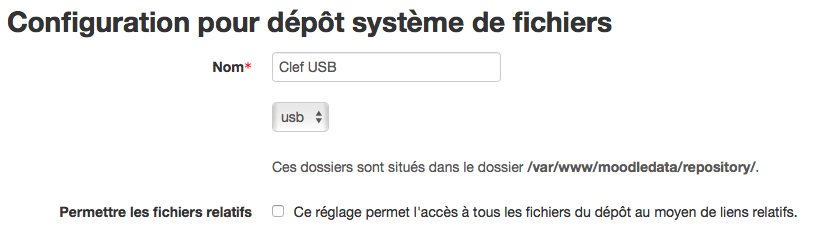
\includegraphics[width=11cm]{repo-filesystem-usb-2.png}
\end{minipage}
\end{figure}

\subsection{Fichiers déposés par SFTP}

On crée un dossier dans lequel les fichiers devront être déposés pour être accessibles depuis Moodle, ainsi qu'un lien vers le dossier de données de Moodle. Les permissions adéquates sont données.

\begin{lstlisting}[language=bash]
$ mkdir -p /home/moodlebox/files
$ sudo chown -R moodlebox:www-data files/
$ sudo chmod g+s files/
$ sudo ln -s /home/moodlebox/files /var/www/moodledata/repository
\end{lstlisting}

On effectue la configuration d'un dépôt \emph{Système de fichiers}, de façon similaire au dépôt « Clef USB » ci-dessus, en indiquant le dossier \emph{files} et en indiquant \emph{Fichiers SFTP} comme nom de dépôt.

Pour déposer des fichiers, on se connecte au moyen d'un logiciel SFTP\footnote{Par exemple : \href{https://filezilla-project.org/}{FileZilla}, \href{https://cyberduck.io/}{Cyberduck}, \href{http://winscp.net/}{WinSCP}.} sur la MoodleBox, avec le nom d'utilisateur \emph{moodlebox} et le mot de passe \emph{Moodlebox4\$}. Les fichiers seront déposés dans le dossier \lstinline{files}.

\section{Configurations additionnelles de Moodle}

\subsection{Activation de l'accès via l'app mobile de Moodle}

Après s'être connecté à la plateforme avec le compte administrateur,  on visite dans le Moodle \emph{Administration du site > Plugins > Services web > Mobile}. On coche la case \emph{Activer les services web pour appareils mobiles} et l'on enregistre les modifications.

Pour cette plateforme dont la destination n'est pas d'être publiée sur Internet, l'avertissement concernant le certificat SSL peut être ignoré sans risque.

\begin{verification}
Depuis un smartphone connecté en Wi-Fi sur le réseau MoodleBox, lancer l'app mobile Moodle et se connecter à la plateforme au moyen de l'URL \url{http://moodlebox.local}, avec le compte administrateur. Aucune erreur ne doit être signalée, et le message \emph{Aucune information de cours à afficher} est affiché sur l'écran du smartphone.
\end{verification}

\subsection{Installation du plugin Administration MoodleBox}

Afin de permettre le redémarrage et l'arrêt de la MoodleBox sans risque de corruption de la carte microSD, ainsi que pour donner des informations utiles sur son fonctionnement, on installe le plugin d'administration \emph{MoodleBox} pour Moodle.

Le plus simple est de l'installer via Git.

\begin{lstlisting}[language=bash]
$ cd /var/www/html/admin/tool/
$ sudo git clone https://github.com/martignoni/moodlebox-plugin.git moodlebox
$ cd /var/www/html/admin/tool/moodlebox
$ sudo touch .reboot-server; touch .shutdown-server; touch .set-server-datetime
$ sudo chown -R www-data:www-data /var/www/html/admin/tool/moodlebox
\end{lstlisting}

On termine l'installation du plugin en visitant la page \url{http://moodlebox.local/admin}. On installe pour terminer le paquetage \emph{incron}.

\begin{lstlisting}[language=bash]
$ sudo apt-get install incron
\end{lstlisting}

On autorise l'utilisation de \emph{incron} par \emph{root}, puis modifie la table des tâches de \emph{incron}.

\begin{lstlisting}[language=bash]
$ echo root | sudo tee -a /etc/incron.allow
$ sudo incrontab -e
\end{lstlisting}

en y ajoutant les lignes
\begin{lstlisting}[language=bash]
/var/www/html/admin/tool/moodlebox/.reboot-server IN_CLOSE_WRITE /sbin/shutdown -r now
/var/www/html/admin/tool/moodlebox/.shutdown-server IN_CLOSE_WRITE /sbin/shutdown -h now
/var/www/html/admin/tool/moodlebox/.set-server-datetime IN_MODIFY /bin/bash /var/www/html/admin/tool/moodlebox/.set-server-datetime
\end{lstlisting}


\section{Configuration de PhpMyAdmin (optionnel)}

\begin{lstlisting}[language=bash]
$ sudo apt-get install phpmyadmin
$ sudo ln -s /usr/share/phpmyadmin /var/www/html/phpmyadmin
\end{lstlisting}
Définir un mot de passe fort. Pour cette installation, le mot de passe choisi est \emph{Moodlebox4\$}.

\begin{verification}
Charger l'URL \url{http://moodlebox.local/phpmyadmin/}. L'interface de PhpMyAdmin doit s'afficher. Pour s'y connecter, utiliser le nom d'utilisateur \emph{root} et le mot de passe \emph{Moodlebox4\$}.
\end{verification}

\section{Optimisation}

Pour que la MoodleBox soit utilisable en pratique, il est nécessaire de prendre soin à son optimisation. On configure ainsi le cache de Moodle, ainsi que sa gestion des dépôts et téléchargements de fichiers.

\subsubsection[Disque RAM pour certains dossiers de Moodle]{Disque RAM pour certains dossiers de Moodle\footnote{Cette section est en partie inspirée de \url{https://www.leading-interactive.de/e-learning/moodle-performance-tuning-mit-tmpfs/}.}}

Créer un dossier comme point de montage pour le disque RAM.
\begin{lstlisting}[language=bash]
$ cd /var/cache/
$ sudo mkdir moodle
$ sudo chown www-data:www-data moodle/
\end{lstlisting}

On utilise également des disques RAM pour le dossier temporaire et le dossiers des sessions de Moodle. Ces deux dossiers sont situés dans le dossier \emph{moodledata}.

On définit dans la table des partitions du Raspberry les disques RAM. Pour ce faire, on ajoute au fichier \lstinline{/etc/fstab}, les lignes suivantes
\begin{lstlisting}[language=bash]
tmpfs /var/cache/moodle tmpfs size=64M,mode=775,uid=www-data,gid=www-data 0 0
tmpfs /var/www/moodledata/temp tmpfs size=64M,mode=775,uid=www-data,gid=www-data 0 0
tmpfs /var/www/moodledata/sessions tmpfs size=32M,mode=775,uid=www-data,gid=www-data 0 0
\end{lstlisting}

%\begin{lstlisting}[language=bash]
%$ sudo nano /etc/fstab
%\end{lstlisting}
%
Le contenu du fichier \lstinline{/etc/fstab} sera alors :
\lstinputlisting[language=bash]{files/fstab}

Après un redémarrage de la Raspberry, le cache peut être configuré dans Moodle.

On se connecte à Moodle avec le compte administrateur (créé plus haut), puis dans le Moodle on visite \emph{Administration du site > Plugins > Cache > Configuration}. On crée deux nouvelles instances de dépôt, en cliquant sur \emph{Ajouter une instance} dans la section \emph{Entrepôts de cache installés} (en haut de la page).

\begin{figure}[!ht]
\begin{minipage}[b]{0.45\linewidth} % A minipage that covers half the page
\centering
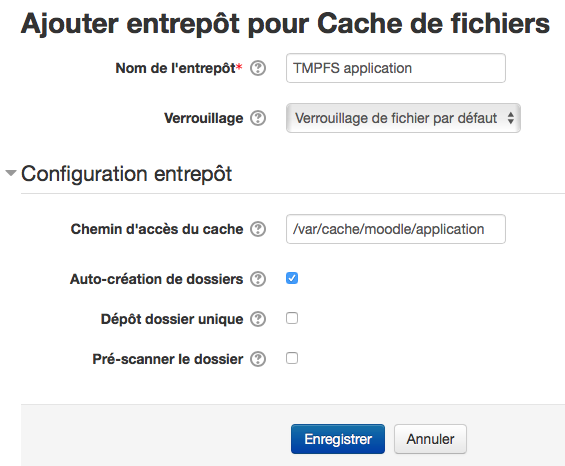
\includegraphics[width=7.3cm]{cache-application.png}
\end{minipage}
\hspace{\fill} % To get a little bit of space between the figures
\begin{minipage}[b]{0.45\linewidth}
\centering
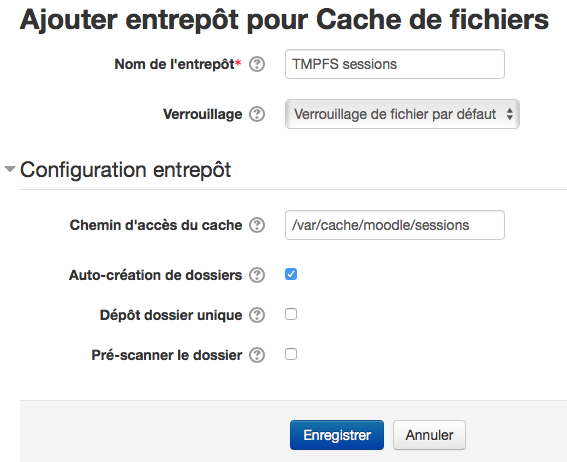
\includegraphics[width=7.3cm]{cache-sessions.png}
\end{minipage}
\end{figure}

\begin{enumerate}
\item Nom de l'entrepôt : \emph{TMPFS application}, chemin d'accès du cache : \emph{/var/cache/moodle/application}, cocher la case \emph{Auto-création de dossiers};
\item Nom de l'entrepôt : \emph{TMPFS sessions}, chemin d'accès du cache : \emph{/var/cache/moodle/sessions}, cocher la case \emph{Auto-création de dossiers}.
\end{enumerate}

Pour terminer, il reste à associer ces nouvelles instances de cache à leur destination, en cliquant sur \emph{Modifier les correspondances} tout en bas de la page, dans le domaine \emph{Entrepôts utilisés en l'absence de correspondance}.

\begin{figure}[!ht]
\begin{minipage}[b]{\linewidth}
\centering
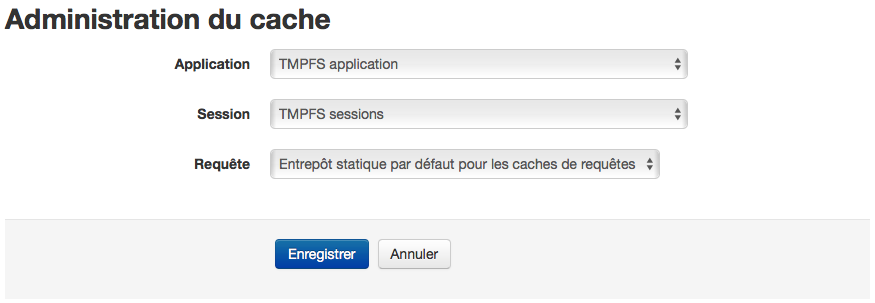
\includegraphics[width=11cm]{cache-association.png}
\end{minipage}
\end{figure}

\begin{verification}
Après quelques actions sur la plateforme Moodle de la MoodleBox, se connecter via SSH à la MoodleBox, puis lancer la commande
\begin{lstlisting}[language=bash]
ls -l /var/cache/moodle/
\end{lstlisting}
La console doit afficher quelque chose comme
\begin{lstlisting}[language=bash]
total 0
drwxrwxrwx 19 www-data www-data 380 mai   30 19:18 application
drwxrwxrwx  8 www-data www-data 160 mai   29 19:00 sessions
\end{lstlisting}
\end{verification}

Le cache en disque RAM a un défaut: les données qu'il contient disparaissent à chaque redémarrage de la MoodleBox. Moodle doit donc à chaque fois reconstruire le cache. Si l'on veut conserver le cache entre les redémarrages, on copie à intervalle régulier le contenu du disque RAM sur la carte microSD, et, lors de chaque démarrage, on effectue l'opération inverse.

On crée le dossier de sauvegarde, puis on définit le cron
\begin{lstlisting}[language=bash]
$ sudo mkdir /var/cache/moodle-cache-backup/
$ sudo crontab -e
\end{lstlisting}

On ajoute à la table des crons les deux lignes suivantes pour effectuer la sauvegarde du cache toutes les 20 minutes et pour restaurer le cache au démarrage:
\begin{lstlisting}[language=bash]
*/20 * * * * rsync -a --delete /var/cache/moodle/ /var/cache/moodle-cache-backup/
@reboot cp -Rpf /var/cache/moodle-cache-backup/* /var/cache/moodle/
\end{lstlisting}

\subsubsection[Utilisation de \emph{X-Sendfile}]{Utilisation de \emph{X-Sendfile}\footnote{Cette section est inspirée de \url{https://moopi.uk/mod/page/view.php?id=81}.}}

L'utilisation de \emph{X-Sendfile} permet d'accélérer l'envoi par le serveur web des fichiers du dossier de données de Moodle.

Ajouter les lignes
\begin{lstlisting}[language=bash]
$CFG->xsendfile = 'X-Accel-Redirect';
$CFG->xsendfilealiases = array (
    '/dataroot/' => $CFG->dataroot
);
\end{lstlisting}
après la ligne \lstinline{$CFG->admin = 'admin';} dans le fichier de configuration de Moodle \lstinline{/var/www/html/config.php}.

%\begin{lstlisting}[language=bash]
%$ sudo nano /var/www/html/config.php
%\end{lstlisting}

Le contenu du fichier \lstinline{/var/www/html/config.php} sera alors :
\lstinputlisting[language=bash]{files/config.php}

Ajouter ensuite les lignes ci-dessous dans le fichier \lstinline{/etc/nginx/sites-available/default}

\begin{lstlisting}[language=bash]
location /dataroot/ {
    internal;
    alias /var/www/moodledata/;
}
\end{lstlisting}

Le contenu du fichier \lstinline{/etc/nginx/sites-available/default} devient alors :
\lstinputlisting[language=bash]{files/default2}

\subsubsection{Optimisation de MySQL}

On modifie les valeurs de quelques variables de MySQL dans le fichier \lstinline{/etc/mysql/my.cnf}. Pour ce faire, on ouvre le fichier en question
%\begin{lstlisting}[language=bash]
%$ sudo nano /etc/mysql/my.cnf
%\end{lstlisting}
et on y modifie les lignes adéquates, à savoir:
\begin{lstlisting}[language=bash]
table_cache             = 512
table_definition_cache  = 512
max_connections         = 100
query_cache_size        = 8M
query_cache_type        = 0
\end{lstlisting}

\section{Nettoyage de la distribution}

Les commandes ci-dessous permettent de nettoyer la MoodleBox et de diminuer l'espace disque qui lui est nécessaire, avant de la cloner et de la distribuer.

\begin{lstlisting}[language=bash]
$ sudo rm -r /var/www/moodledata/cache/*
$ sudo rm -r /var/www/moodledata/localcache/*
$ sudo rm -r /var/www/moodledata/temp/*
$ sudo rm -r /var/www/moodledata/trashdir/*
$ sudo rm -r /var/www/moodledata/sessions/*
$ sudo rm -r /var/cache/moodle/*
$ sudo rm -r /var/cache/moodle-cache-backup/*
$ mysql -u root -p'Moodlebox4$' moodle -e "truncate table moodle.mdl_logstore_standard_log"
$ mysql -u root -p'Moodlebox4$' moodle -e "truncate table moodle.mdl_config_log"
$ sudo apt-get clean
$ sudo rm -r /var/cache/debconf/*
$ sudo rm -r /tmp/*
$ sudo rm -r /var/tmp/*
$ rm ~/.mysql_history
$ sudo bash -c 'for logs in `find /var/log -type f`; do > $logs; done'
$ cat /dev/null > ~/.bash_history && history -c && sudo shutdown -h now
\end{lstlisting}

Si tout s'est bien passé, la totalité ne doit pas dépasser la taille de 1.8~Go. L'image-disque, une fois tronquée, a une taille d'envion 2.5~Go. Compressée, elle tient dans un peu plus d'1~Go.


\end{document}
%%